\documentclass{article}
\usepackage[title]{appendix}
\usepackage{authblk}
\usepackage{mathptmx}
\usepackage{url,latexsym,amsmath,amsthm,xspace,rotating,multirow,multicol,xspace,amssymb,paralist}
\usepackage{euscript}
\usepackage{fancybox,xcolor}
\usepackage{longtable}
\usepackage{paralist}
\usepackage[normalem]{ulem}
\usepackage{algorithmicx}
\usepackage{algpseudocode}
\usepackage{algorithm}
\usepackage{cancel}
\usepackage{mathtools}
\usepackage{fullpage}
\usepackage[nodayofweek]{datetime}
\usepackage{subfig}


\usepackage{url}
\usepackage{latexsym}
\usepackage{media9}

\usepackage{times}
\usepackage{amsmath}
\usepackage{amsthm}
\usepackage{amssymb}
\usepackage{graphicx}
\graphicspath{ {images/} }
\usepackage{xspace}
\usepackage{tabularx}
\usepackage{multicol}
\usepackage{multirow}
%\usepackage{hyperref}
\usepackage{url}
%\usepackage{natbib}
\usepackage{wrapfig}
\usepackage{comment}
\usepackage{listings}
\usepackage{color}
\usepackage[utf8]{inputenc}
\usepackage{fancyvrb}
\usepackage{booktabs}
\usepackage{color}
\usepackage[normalem]{ulem}

\usepackage{textcomp}

\newcommand{\obs}{\text{obs}}
\newcommand{\mis}{\text{mis}}

\newcommand{\qt}[1]{\left<#1\right>}
\newcommand{\ql}[1]{\left[#1\right]}
\newcommand{\hess}{\mathbf{H}}
\newcommand{\jacob}{\mathbf{J}}
\newcommand{\hl}{HL}
\newcommand{\cost}{\mathcal{L}}
\newcommand{\lout}{\mathbf{r}}
\newcommand{\louti}{r}
\newcommand{\outi}{y}
\newcommand{\out}{\mathbf{y}}
\newcommand{\gauss}{\mathbf{G_N}}
\newcommand{\eye}{\mathbf{I}}
\newcommand{\softmax}{\text{softmax}}
\newcommand{\targ}{\mathbf{t}}
\newcommand{\metric}{\mathbf{G}}
\newcommand{\sample}{\mathbf{z}}
\newcommand{\f}{\text{f}}
%\newcommand{\log}{\text{log}}

\newcommand{\bmx}[0]{\begin{bmatrix}}
\newcommand{\emx}[0]{\end{bmatrix}}
\newcommand{\qexp}[1]{\left<#1\right>}
\newcommand{\vect}[1]{\mathbf{#1}}
\newcommand{\vects}[1]{\boldsymbol{#1}}
\newcommand{\matr}[1]{\mathbf{#1}}
\newcommand{\var}[0]{\operatorname{Var}}
\newcommand{\std}[0]{\operatorname{std}}
\newcommand{\cov}[0]{\operatorname{Cov}}
\newcommand{\diag}[0]{\operatorname{diag}}
\newcommand{\matrs}[1]{\boldsymbol{#1}}
\newcommand{\va}[0]{\vect{a}}
\newcommand{\vb}[0]{\vect{b}}
\newcommand{\vc}[0]{\vect{c}}
\newcommand{\ve}[0]{\vect{e}}

\newcommand{\vh}[0]{\vect{h}}
\newcommand{\vv}[0]{\vect{v}}
\newcommand{\vx}[0]{\vect{x}}
\newcommand{\vp}[0]{\vect{p}}
\newcommand{\vz}[0]{\vect{z}}
\newcommand{\vw}[0]{\vect{w}}
\newcommand{\vs}[0]{\vect{s}}
\newcommand{\vf}[0]{\vect{f}}
\newcommand{\vi}[0]{\vect{i}}
\newcommand{\vo}[0]{\vect{o}}
\newcommand{\vd}[0]{\vect{d}}
\newcommand{\vy}[0]{\vect{y}}
\newcommand{\vg}[0]{\vect{g}}
\newcommand{\vm}[0]{\vect{m}}
\newcommand{\vu}[0]{\vect{u}}
\newcommand{\vL}[0]{\vect{L}}
\newcommand{\vr}[0]{\vect{r}}
\newcommand{\vone}[0]{\vect{1}}

\newcommand{\mW}[0]{\matr{W}}
\newcommand{\mE}[0]{\matr{E}}
\newcommand{\mG}[0]{\matr{G}}
\newcommand{\mX}[0]{\matr{X}}
\newcommand{\mY}[0]{\matr{Y}}
\newcommand{\mQ}[0]{\matr{Q}}
\newcommand{\mB}[0]{\matr{B}}
\newcommand{\mU}[0]{\matr{U}}
\newcommand{\mF}[0]{\matr{F}}
\newcommand{\mV}[0]{\matr{V}}
\newcommand{\mA}{\matr{A}}
\newcommand{\mC}{\matr{C}}
\newcommand{\mD}{\matr{D}}
\newcommand{\mL}[0]{\matr{L}}
\newcommand{\mR}[0]{\matr{R}}
\newcommand{\mS}{\matr{S}}
\newcommand{\mI}{\matr{I}}
\newcommand{\td}[0]{\text{d}}
\newcommand{\TT}[0]{\vects{\theta}}
\newcommand{\vsig}[0]{\vects{\sigma}}
\newcommand{\valpha}[0]{\vects{\alpha}}
\newcommand{\vmu}[0]{\vects{\mu}}
\newcommand{\vzero}[0]{\vect{0}}
\newcommand{\tf}[0]{\text{m}}
\newcommand{\tdf}[0]{\text{dm}}
\newcommand{\grad}[0]{\nabla}
\newcommand{\alert}[1]{\textcolor{red}{#1}}
\newcommand{\N}[0]{\mathcal{N}}
\newcommand{\YY}[0]{\mathcal{Y}}
\newcommand{\BB}[0]{\mathcal{B}}
\newcommand{\LL}[0]{\mathcal{L}}
\newcommand{\HH}[0]{\mathcal{H}}
\newcommand{\RR}[0]{\mathbb{R}}
\newcommand{\MM}[0]{\mathcal{M}}
\newcommand{\OO}[0]{\mathbb{O}}
\newcommand{\II}[0]{\mathbb{I}}
\newcommand{\Scal}[0]{\mathcal{S}}
\newcommand{\sigmoid}{\sigma}
\newcommand{\sign}{\text{sign}}
\newcommand{\E}[0]{\mathbb{E}}
\newcommand{\enabla}[0]{\ensuremath{%
    \overset{\raisebox{-0.3ex}[0.5ex][0ex]{%
    \ensuremath{\scriptscriptstyle e}}}{\nabla}}}
\newcommand{\enhnabla}[0]{\nabla_{\hspace{-0.5mm}e}\,}
\newcommand{\eos}[0]{\ensuremath{\left< \text{eos}\right>}}


\newcommand{\todo}[1]{{\Large\textcolor{red}{#1}}}
\newcommand{\done}[1]{{\Large\textcolor{green}{#1}}}
\newcommand{\dd}[1]{\ensuremath{\mbox{d}#1}}

\DeclareMathOperator*{\argmax}{\arg \max}
\DeclareMathOperator*{\argmin}{\arg \min}
\newcommand{\newln}{\\&\quad\quad{}}

\newcommand{\BP}{\text{BP}}
\newcommand{\PPL}{\text{PPL}}
\newcommand{\PL}{\text{PL}}
\newcommand{\MatSum}{\text{MatSum}}
\newcommand{\MatMul}{\text{MatMul}}
\newcommand{\KL}{\text{KL}}
\newcommand{\data}{\text{data}}
\newcommand{\rect}{\text{rect}}
\newcommand{\maxout}{\text{maxout}}
\newcommand{\train}{\text{train}}
\newcommand{\hinge}{\text{hinge}}
\newcommand{\val}{\text{val}}
\newcommand{\init}{\text{init}}
\newcommand{\fenc}{\text{fenc}}
\newcommand{\renc}{\text{renc}}
\newcommand{\enc}{\text{enc}}
\newcommand{\dec}{\text{dec}}
\newcommand{\test}{\text{test}}
\newcommand{\tra}{\text{tra}}
\newcommand{\Ax}{\mathcal{A}_x}
\newcommand{\Ay}{\mathcal{A}_y}
\newcommand{\ola}{\overleftarrow}
\newcommand{\ora}{\overrightarrow}
\newcommand{\ov}{\overline}
\newcommand{\ts}{\rule{0pt}{2.6ex}}       % Top strut
\newcommand{\ms}{\rule{0pt}{0ex}}         % Middle strut
\newcommand{\bs}{\rule[-1.2ex]{0pt}{0pt}} % Bottom strut
\newcommand{\specialcell}[2][c]{%
  \begin{tabular}[#1]{@{}c@{}}#2\end{tabular}}


%\usepackage{bibentry}
%\nobibliography*

\begin{document}
\title{Ride-Sharing Routes in a City}
\author{Aidan Claffey}
\date{\today}
\maketitle

\section{Introduction}
In the past five years, ride-sharing apps have exploded onto the global economy, with Uber leading the way. Recently, in New York City and, I imagine in other cities, traffic has gotten worse. No doubt this is partially due to the increase in ride-sharing app use (also due to the MTA failure, at least in New York City). Thus, the apps themselves, and cities as a whole, are trying to figure out new ways to accommodate the increase in traffic. My model, building off of the basic traffic model discussed in class, has ride-sharing cars that wander around the city picking up and dropping off passengers while normal cars get in their way. To make things easier, I will refer to ride-sharing cars as \textit{ubers}.

\section{The environment}
\subsection{The city}
The city that I have set the cars up in is a six-by-six grid, where the the horizontal blocks are 0.2 miles and the vertical blocks are 0.4 miles. In this paper I will refer to the vertical streets as \textit{avenues} and the horizontal streets as \textit{streets}. The first, third, and fifth avenues counting from the left) run north to south while the second, fourth, and sixth run south to north. The first, third, and fifth streets (counting from the bottom) run west to east while the second, fourth, and sixth streets run east to west. Additionally, there is what I call a \textit{beltway} running counter-clockwise around the city that connects at each corner. All streets and avenues have a speed limit of 25 mph and the beltway has a speed limit of 60 mph.

\begin{figure}[h]
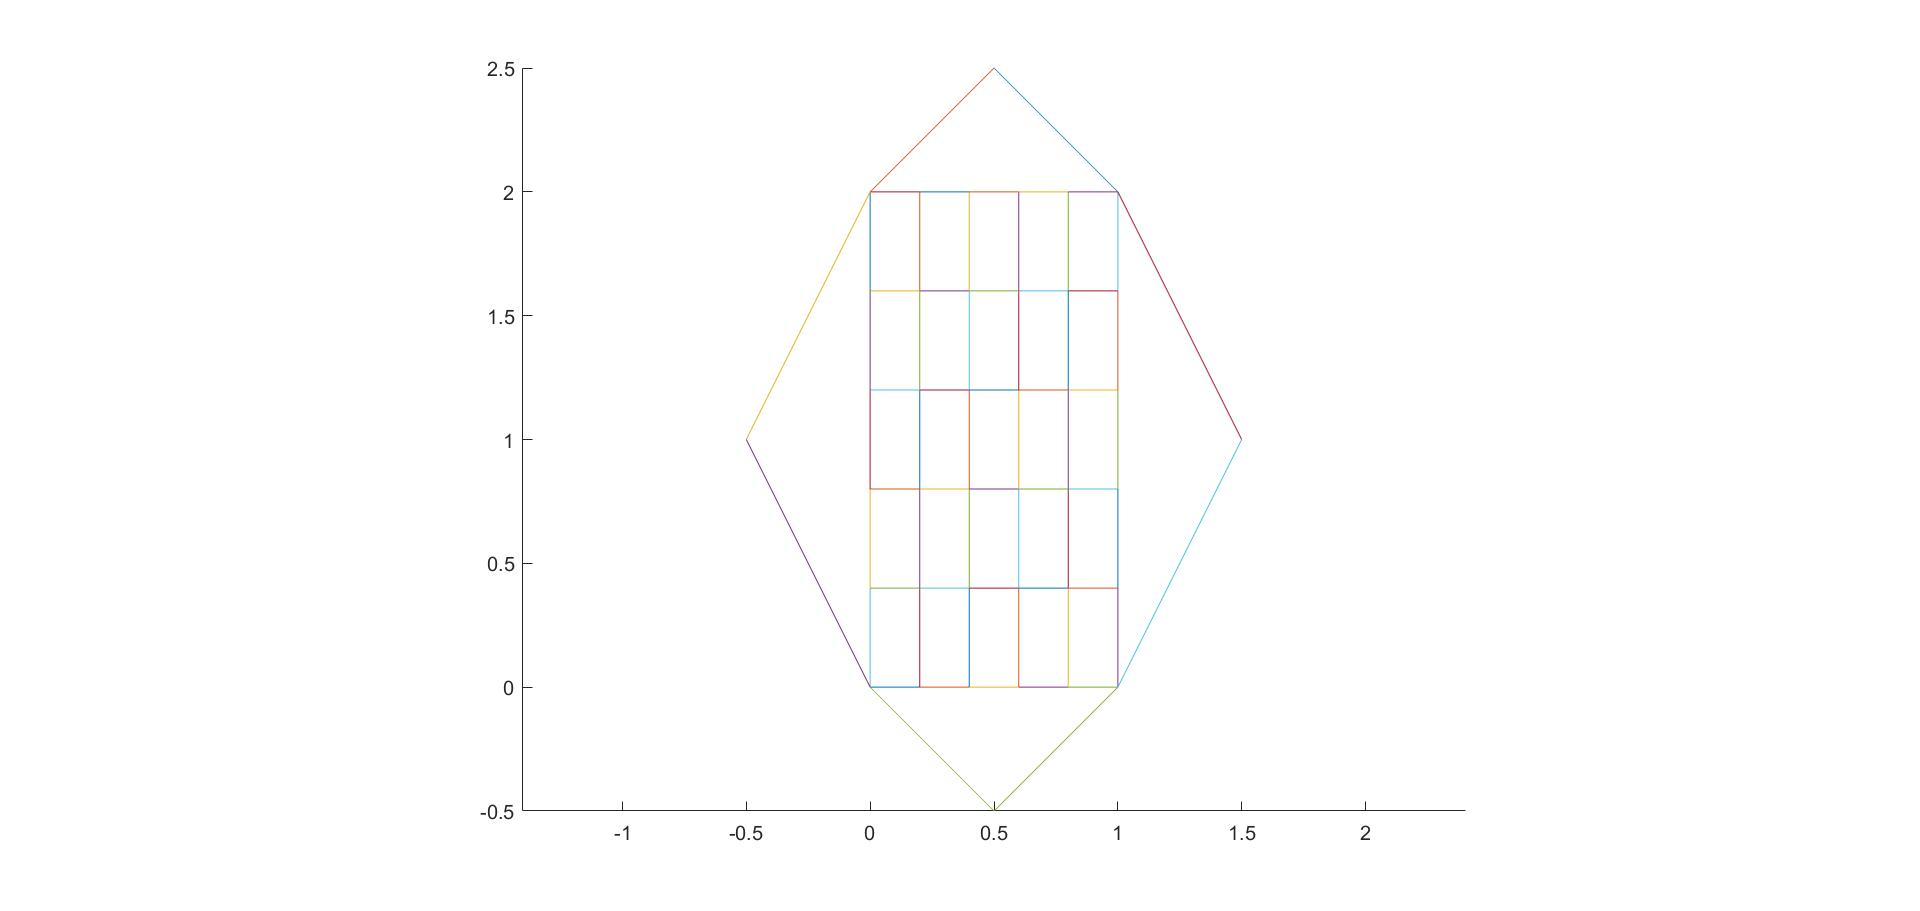
\includegraphics[width=16cm]{mapofcity.jpg}
\end{figure}

\subsection{Driving around the city}
\subsubsection{Traffic lights}
Each block going into an intersection has a traffic light which is either green or red. Only one incoming block at each intersection has a green light while the rest have red-lights. Therefore, if there is only one incoming block, it is green all the time. Traffic lights within an intersection rotate with a specified time step (i.e. no "smart" traffic lights that change due to the number of cars waiting), which in this model is 30 seconds.

\subsubsection{Determining speed}
As discussed in class, cars follow a velocity function based on the distance to either the car, the red light, or the destination ahead of the car, which is given by $d$. It also depends on the constants for speed limit ($v_{max}$) and two variables called $d_{min}$ and $d_{max}$, where $d_{min}$ is closest the car will get to a traffic light or car ahead before coming to a complete stop, and $d_{max}$ is distance at which a car does not take into account the car (or traffic light) ahead.
\[V(d) = \begin{cases} 
      	v_{max} & d > d_{max}\\
      	v_{max} \dfrac{\ln{\dfrac{d}{d_{min}}}}{\ln{\dfrac{d_{max}}{d_{min}}}} & d_{max} \leq d \geq d_{min}\\
      	0 & d < d_{min} 
   	\end{cases}\]

Thus, there is no possibility for car crashes or accidents in this model, as there is no acceleration function.

\subsubsection{Turning}
When turning, cars in this model have the ability to look at the slowest car on the block they are turning on and adjusting speed based on that distance using the velocity function above.

\subsection{Uber-specific rules}
\subsubsection{The passengers}
While normal cars drive around picking their turns at random, ubers have a job to do! Passengers will randomly pop up at any point on the city grid (they cannot appear on the beltway) and each passenger has a randomly assigned destination, also on the city grid. An uber is assigned a passenger using a method described below.

\subsubsection{Finding an uber}
Essentially, ubers are assigned to passengers based on proximity and number of passengers in the uber's queue. First the model looks for ubers with the lowest number of passengers in its queue. Then, one of two scenarios happen:
\begin{enumerate}
\item If the subset of ubers has a queue length of zero (i.e. the uber does not have a passenger in its car and it is not on the way to pick up anyone, then the uber that is closest (using euclidean distance) to the intersection that the passenger's block begins at adds that passenger to its queue.
\item If the subset of ubers has a queue length $n$ > $0$, then the uber selected is the one who's $n-1$th passenger's destination is closest to the passenger.
\end{enumerate}
Although this is not the most efficient way to assign ubers, it was the simplest to implement while making sure passengers did not wait too long.

\section{Choosing the route - Results}
Whether driving to pick up the passenger or driving the passenger to its destination, the uber needs to know where to go. It chooses the path to go using MATLAB's function \textit{graphshortestpath}, which uses the classic shortest path algorithm, Dijkstra's Algorithm. The algorithm requires a starting vertex, an ending vertex, and a graph with weights. The weights are assigned in between two connected nodes and are used to determine the shortest path. In my model, I set weights in several different ways and tested the efficiency of the model based on the different ways to set weights. An efficient model is one that has the lowest average "wait time" for passengers from the time they are created to the time they are picked up.
\section{Methods and results}
See videos attached to the email for demonstrations for different path optimizing methods
\subsection{Method one: distance as weights}
Weights for this method were determined based on the distance between two connected blocks. Displayed below is the path an uber would take from the top left corner to the bottom right corner using this method.

Here are the weights for each type block
 
\begin{center}
\begin{tabular}{ |c|c| } 
 \hline
 \textit{block type} & \textit{weight} \\ 
 horizontal & 0.2 mi \\ 
 vertical & 0.4 mi\\
 east and west beltway & 1.1180 mi\\
 north and south beltway & 0.7071 mi\\
 \hline
\end{tabular}
\end{center}

\subsection{Methods two, three, and four: expected time as weights}
Weights in between nodes were also calculated using the expected time it would take for a car to travel on a block.
\subsubsection{Using the speed limit}
Expected time for a car to cross a section of road can be easily determined by dividing the length of the road by the speed limit for that road. Weights are shown below 
 
\begin{center}
\begin{tabular}{ |c|c|c| } 
 \hline
 \textit{block type} & \textit{speed limit}  & \textit{weight}\\ 
 horizontal & 25 mph & .0080 hr\\ 
 vertical & 25 mph & .0160 hr\\
 east and west beltway & 60 mph & .0146 hr\\
 north and south beltway & 60 mph & .0118 hr\\
 \hline
\end{tabular}
\end{center}

\subsubsection{Using the speed limit and traffic lights}
A more complicated way to measure expected time for a car to travel across a block is to not only take into account the speed limit and the distance, but to account for the number of traffic lights for the intersection as well. For example, an intersection that has two blocks going into is going to only allow one of the two blocks in at a time, so those two blocks are going to take, on average, slower than blocks of the same length and speed limit, but no traffic light. So, to account for this, I found the expected time calculation for a car to cross a block given its traffic light condition:

Let:
\begin{itemize}
	\item $L =$ the length of the block
	\item $b$ the number of blocks entering the intersection that the block is entering 
\end{itemize}

\[ E[t] = \dfrac{(L - d_{max})}{v_{max}} + P(\text{light is green})\dfrac{d_{max}}{v_{max}} + P(\text{light is red})\dfrac{d_{max}}{\text{average velocity given red light}}\]

where the probabilities for red and green lights are given by:
\[P(\text{green light}) = 1 - P(\text{red light}) = \dfrac{1}{b}\]

and where the average velocity given a red light from 0 to $d_{max}$ is given by:
\[v_{max}\dfrac{1}{d_{max}} \int_{d_{min}}^{d_{max}} v(d) dd\]
\[= v_{max}\dfrac{d_{min}}{d_{max}}\]

So, weights for each type of block look like:
\begin{center}
\begin{tabular}{ |c|c|c| } 
 \hline
 \textit{block type} & \textit{number of blocks entering intersection}  & \textit{weight}\\ 
 horizontal & 1 & .0080 hr\\
 horizontal & 2 & .0148 hr\\ 
 vertical & 1 & .0160 hr\\
 vertical & 2 & .0228 hr\\
 east and west beltway & 1 & .0146 hr\\
 east and west beltway & 2 & .0215 hr\\
 north and south beltway & 1 & .0 hr\\
 north and south beltway & 2 & .0160 hr\\
 \hline
\end{tabular}
\end{center}

\subsubsection{Trying to optimize for traffic}
I also tried to calculate weights by accounting for traffic. I did this by calculating the average velocity of the cars on each block, and used the distance of the block divided by the average velocity as the weights for Dijkstra's Algorithm.

\subsection{Results}
For 100 runs of each model, I calculated the average wait time for each passenger. The results are as follows:

\begin{center}
\begin{tabular}{ |c|c| } 
 \hline
 \textit{MODEL} & \textit{AVG. WAIT TIME} \\ 
 Distance & 0.1754 hours \\ 
 Speed Limit w/o traffic lights & 0.1495 hours\\
 Speed Limit w/ traffic lights & 0.1584 hours\\
 Traffic &  0.1530 hours\\
 \hline
\end{tabular}
\end{center}

The results demonstrate that adjusting the weight using traffic lights does not help, and actually slows down the model. Additionally, as expected, the Distance model was the least efficient, since ubers using this method would never use the beltway. Also, the traffic model did slightly better than the model that takes into account traffic lights, but slightly worse than just the speed limit model. Overall, it seems that trying to overcomplicate the shortest path calculations actually makes the model perform slightly worse, although given the randomness of the model, the differences between the three best performing models is not large enough to say definitively which is the best.

\section{Additional Exploration: Another beltway}
I wanted to see if adding another beltway going the opposite direction as the original beltway would make traffic more efficient. Since the BLANK method is the most efficient in the single-beltway model, I only expanded on this model to see whether an additional beltway makes a difference. As it turns out, it BLANK.

Here are the results:
\begin{center}
\begin{tabular}{ |c|c| } 
 \hline
 \textit{MODEL} & \textit{AVG. WAIT TIME}\\ 
 Single Beltway & 0.1495 hours\\ 
 Double Beltway & 0.1562 hours\\
 \hline
\end{tabular}
\end{center}

As you can see adding the second beltway does not increase the efficiency of the model, counterintuitively. 

\section{Limitations and Extensions}
This model is a very abstract model of a city, especially given the size of the city. Additionally, ridesharing apps do not work like this in reality, instead, the driver of a ridesharing car can choose to accept or not accept a request from a passenger. However, the model itself is very expandable, and many extensions can be done to make the model more realistic. Here are a few:
\begin{itemize}
	\item Do real-time updates of a route based on current traffic conditions
	\item Increase the size of the city and make certain districts have passengers than others (like a residential vs business district
	\item have two competing ride-share models that have different algorithms and see which performs better real-time
\end{itemize}

\section{code}
I chose to only include some of the source code, since it would be way too long if I included all of it. The finduber.m file demonstrates how a new passenger is assigned an uber.
\begin{lstlisting}[language = matlab]
%mainprogram: The script that runs the code
npmax = 50;
numruns = 100;
average_timepickedup = zeros(1, npmax);

for run = 1:numruns
    %main program:
    initialize %this is where you initialize the state
    insertubers
    plotcars
    axis equal
    pause(5)
    for clock = 1:clockmax
        if(npdroppedoff <=npmax)
            t = clock * dt;
            setlights
            createpassengers
            movecars
            plotcars
            axis equal
            round = clock;
        end
    end

    average_timepickedup = average_timepickedup + tpickedup - tenter;
end
bar(average_timepickedup / numruns)
mean(average_timepickedup)/numruns
\end{lstlisting}

\begin{lstlisting}[language = matlab]
% # of ubers, constant
nu = 10;

% # of random cars
nrandomcars = 100;

%Number of passengers, initially
np = 0;

%uber that the passenger will take
uber = zeros(1, np);
%passenger that is in the uber
passenger = zeros(1, nu);

% # of max passengers allowed
nptot = 0;
npdroppedoff = 0;
% # of intersections
ni = 44;
% # of blocks
nb = 76;
%distance behind next car such that car will go 0 or max speed
dmin = 20/5280; %20 feet in miles
dmax = 200/5280; % 200 feet
vmax = zeros(1, nb); %speed limit of 40
vmax(1:60) = 25;
vmax(61:68) = 60;
vmax(69:76) = 60;

%block array indices:
%block array indices:
i1 = [1 2 3 4 5 7 2 9 4  11 6  8 9 10 11 12 13 8  15 10 17 12 13 14 15 16 17 19 14 21 16 23 18];
i2 = [2 3 4 5 6 1 8 3 10 5  12 7 8 9  10 11 7  14 9  16 11 18 14 15 16 17 18 13 20 15 22 17 24];

i1(34:55) = [20 21 22 23 24 25 20 27 22 29 24 25 26 27 28 29 31 26 33 28 35 30];
i2(34:55) = [19 20 21 22 23 19 26 21 28 23 30 26 27 28 29 30 25 32 27 34 29 36];

i1(56:60) = [32 33 34 35 36];
i2(56:60) = [31 32 33 34 35];

i1(61:68) = [37 6  38 36 39 31 40 1];
i2(61:68) = [6  38 36 39 31 40 1  37];

i1(69:76) = [6  42 36 43 31 44 1  41];
i2(69:76) = [41 6  42 36 43 31 44 1];
%creategrid
%for mapping an (i1, i2) pair to its vector
i1i2toblock = sparse(i1,i2,1:nb);

nbin = zeros(1, ni);
nbout = zeros(1, ni);

%initialize all blocks
for i = 1:ni
	nbin(i) = sum(i2 == i);
	nbout(i) = sum(i1 == i);
end

nbinmax = max(nbin);
nboutmax = max(nbout);

bin = ones(ni, nbinmax);
bout = ones(ni, nboutmax);

for i = 1:ni
	bin(i, 1:nbin(i)) = find(i2 == i); %where find(i2 == i) makes a list of all i2 that equal i
	bout(i, 1:nbout(i)) = find(i1 == i); 
end

%initialize all traffic lights
jgreen = ones(1, ni);
S = zeros(1, nb);
for i = 1:ni
	b = bin(i,jgreen(i));
    S(b) = 1;
end

%initialize geometric positions of traffic lights
%xi = zeros(ni); yi = zeros(ni)
i=1;
while i <= ni - 4 
    xi(i:i+5) = [0 .2 .4 .6 .8 1];
    yi(i:i+5) = (i-1)/6 * 0.4;
    i = i+6;
end
xi(37:40) = [0.5 1.5 0.5 -0.5];
yi(37:40) = [-0.5 1 2.5 1];

xi(41:44) = [0.5 1.5 0.5 -0.5];
yi(41:44) = [-0.5 1 2.5 1];

%unit vectors for each block
ux = zeros(1, nb); uy = zeros(1, nb);L = zeros(1, nb);
for b = 1:nb
    ux(b) = xi(i2(b)) - xi(i1(b));
	uy(b) = yi(i2(b)) - yi(i1(b));
	L(b) = sqrt(ux(b)^2 + uy(b)^2);
	ux(b) = ux(b)/L(b);
	uy(b) = uy(b)/L(b);
end
Lmax = max(L);

%position of cars
xu = zeros(1, nu + nrandomcars);
yu = zeros(1, nu + nrandomcars);
bu = zeros(1, nu + nrandomcars);
%position of passengers in beginning
xp = zeros(1, npmax);
yp = zeros(1, npmax);
%queue size and queue array
uberqueuesize = zeros(1, nu);
uberqueue = zeros(nu, npmax);

%TODO
%Implement initializations of ubers


hold on
% plot(xplotperim, yplotperim);
% plot(xplotmid1, yplotmid1);
% plot(xplotmid2, yplotmid2);

for i = 1:nb
    plot([xi(i1(i)) xi(i2(i))], [yi(i1(i)) yi(i2(i))])
end

hubers = plot(0, 0, 'o', 'MarkerFaceColor', 'b');
hcars = plot(0, 0, 'o', 'MarkerFaceColor', 'c');
hdestinations = plot(0, 0, 'o', 'MarkerFaceColor', 'g');
hpickupspot = plot(0, 0, 'o', 'MarkerFaceColor', 'r');

hold off

showdestination(1) = 0;
pickedup(1) = 0;

%set max for clock
clockmax = 3600; %1 hour
dt = 1/3600; %one second

%set time for lights to change
tlcstep = 1/120;
tlc = tlcstep;

%initialize linked list system for cars
firstcar = zeros(1, nb);
lastcar = zeros(1, nb);
nextcar = zeros(1, nu + nrandomcars);
%position of car on block
p = zeros(1, nu);

%passengers on the road
onroad = zeros(1, npmax);

%initialize a probabilty under which a car will make a random turn
prchoice = 0.9;

%destination initialization for passengers
bdp = zeros(1, npmax);
pdp = zeros(1, npmax);
xdp = zeros(1, npmax);
ydp = zeros(1, npmax);

%destination initialization for cars
bd = zeros(1, nu);
pd = zeros(1, nu);
xd = zeros(1, nu);
yd = zeros(1, nu);

%for shortest path optimization
distance = zeros(1, length(i1));
for j = 1:length(i1)
    distance(j) = sqrt((xi(i2(j)) - xi(i1(j)))^2 + (yi(i2(j)) - yi(i1(j)))^2);
end
graph = sparse(i1, i2, distance./vmax);


%path will contain the path (in an array of indices), that the car is
%supposed to take
%turn number is the turn that the car is on
path = cell(1, nu);
turnnumber = zeros(1, nu);

startmovingtime = zeros(1, nu + nrandomcars);
\end{lstlisting}

\begin{lstlisting}[language = matlab]
%finduber.m
%finds an uber for the passenger
%rules are: first check for closest uber with no passengers
%if all ubers have a passenger, choose uber with lowest # of passengers
%in queue who's distance from the destination to the new passenger is the
%smallest
minqueuesize = min(uberqueuesize);

distancetopassenger = zeros(1, nu);
%if queue is 0, find closest uber
if minqueuesize == 0
    for u = 1:nu
        if (uberqueuesize(u) > minqueuesize)
            distancetopassenger(u) = Inf;
        else
            distancetopassenger(u) = (xu(u) - xp(np))^2 + (yu(u) - yp(np))^2;
        end
    end
else
    for u = 1:nu
        if uberqueuesize(u) > minqueuesize
            distancetopassenger(u) = inf;
        else
            distancetopassenger(u) = (xdp(uberqueue(u,minqueuesize)) - xp(np))^2 + ...
                (ydp(uberqueue(u,minqueuesize)) - yp(np))^2;
        end 
    end
end

[mindistance, uber(np)] = min(distancetopassenger);

%now, either give uber new passenger or add to queue

if minqueuesize == 0
    xd(uber(np)) = xp(np); yd(uber(np)) = yp(np); bd(uber(np)) = benter(np); pd(uber(np)) = pp(np);
    %if it is a new customer, uber needs a new path
    %two cases for whether destination is on the same block as uber or not
    %this is becuase the getshortestpath matlab function, when given the
    %same point, twice, gives as the shortest path the point
    
    %if same block
    path{uber(np)} = [getshortestpath(graph, i2(bu(uber(np))),... 
                                            i1(benter(np))) bd(uber(np))];
    turnnumber(uber(np)) = 1;
    nextb(uber(np)) = bu(uber(np));
end

uberqueuesize(uber(np)) = uberqueuesize(uber(np)) + 1;
uberqueue(uber(np), minqueuesize + 1) = np;
\end{lstlisting}
\end{document}